\chapter{Taxes}%
\label{chpt:taxes}

Are taxes too high? Here I think that the conservatives are just right: taxes
are too high. However, many of them are wrong on whom they are too high: they
are too high for low-income earners!

We need to distinguish between \emph{average} and \emph{marginal} tax rates.
The \emph{average} tax is very simple: take the amount that you earn pre-taxes,
the amount that went to taxes and divide one by the other. For example, if your
employer spends \$100,000 to hire you; while you get \$70,000 at the end of the
year, then 30,000 or 30\% went to taxes. Your marginal tax rate is how much
taxes you will be paying on your next \$1,000. This is often a very different
number. If your next \$1,000 only net you \$600, then your marginal rate is
40\%. % FIXME Check these values for plausibility

Unfortunately, things can get very complicated very fast as you are taxed in
more ways than just through the tax system. If you lose the right to subsidized
child care for you toddler or to cheaper health insurance as you cross an
income threshold, then your tax rate might be very high.
% Get examples from studies

\section{Are Taxes Too High (on Low-incomes)?}

In early 2013, the Sun newspaper, a vaguely conservative British tabloid,
featured a couple, ``Danny Creamer, 21, and Gina Allan, 18, spend each day
watching their 47in flatscreen TV and smoking 40 cigarettes between them in
their comfy two-bedroom flat.''\footnote{The original piece is available at
\url{http://www.thesun.co.uk/sol/homepage/news/4764841/Why-work.html}.} They
live this lifestyle without working, simply on public benefits.

Naturally, the comments on right-wing blogs debated the immorality of (1) this
pair and (2) the system that allows them to live like this without working.
Most grating were their comments where they portraid themselves as victims,
being ``trapped'' by the system.

The couple may be cheating a little bit (for example, they benefit from a
``Jobseeker's Allowance,'' the term for unemployment insurance in the UK, while
clearly not seeking a job). Their behavior, however, is a perfect example of
what conservatives mean when they say that high taxes discourage work. This
young couple is responding to the immoral incentives that the system puts them
in. It applies to low incomes as much as to the mythical small business owner.
In fact, over the short term, a low-income couple such as this one may fact
effective marginal tax rates of 75\% or more (including marginal rates of over
100\%!).

If high marginal tax rates are bad for high incomes, they are bad for low
incomes too. And if you think that the problem above only happens in the
British system, then think again. The graph on
Figure~\ref{fig:cbo-effective-tax-rate} is the effective tax rate computed by
the Congressional Budget Office.

\begin{figure}
\begin{center}
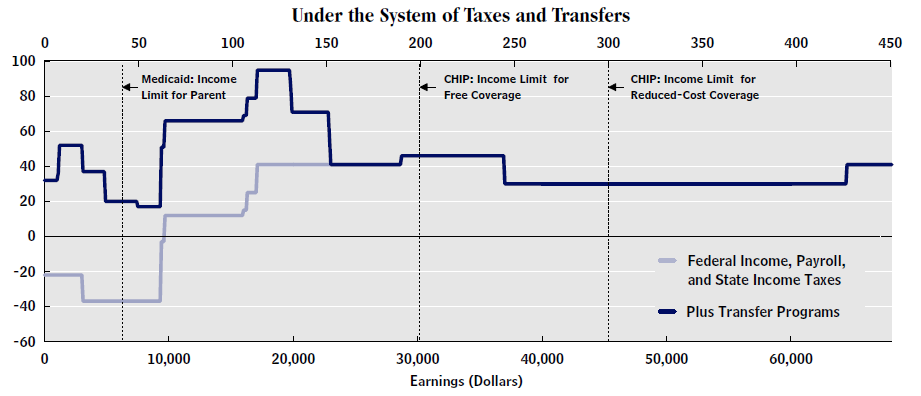
\includegraphics[width=.8\textwidth]{images/cbo-effective-tax-rate.png}
\end{center}
\caption{Effective Tax Rates. These are the effective tax rates computed by the
Congressional Budget Office in the United States.}
\label{fig:cbo-effective-tax-rate}
\end{figure}

\section{Simpler, Flatter, Fairer}

Flat taxes have got a bad reputation as being unfair. To a large extent, this
stems from a misunderstanding of what a flat tax is. What is is flat is not the
\emph{average}, but rather the \emph{marginal} tax rate. If we add a large
deductable, we get a tax-system which \emph{is more progressive than the
current one}.

As Greg Mankiw has written, the current systems is, in fact if not in spirit, a
flat tax system. In fact, the current systems is \emph{much more of a flat tax
system than most so called flat tax systems}.
% http://gregmankiw.blogspot.pt/2012/11/the-us-has-flat-tax-in-effect.html

The only problem with this proposal is that it is politically naïve. The
argument goes something like the following: it will never pass in the United
States, where thousands of interest groups each like their small benefit.
However, at some point in the not-so-distant future, the tax system will need
to change so that it collects more money. At that time, change will come. We
can only try to put good ideas out there so that they may then get picked up,
instead of the idea that was seriously discussed in January 2013 of minting a
trillion dollar coin.\footnote{I actually think it might have been a good idea
to mint that coin as a type of monetary policy, but why not do it properly
through a more active role for monetary policy coming from the Federal
Reserve?}

In Sweden, for most people, taxes are precomputed by the government based on
filings by others (your employer and finantial institutions). Then, the
government sends you their estimate. You have the option of just accepting it
or submitting your own filing. Of course, small business owners or those who
freelance and have many clients may need to file separately, but for over 90\%
of people, the government's estimate will be acceptable. The result is that the
time it takes to do your taxes is about 30~minutes or less. Remember, doing
taxes is a tax too.\footnote{How many hours are wasted on this activity? Even
with software like Turbo Tax (which itself charges a small fee), too much
effort is spent on taxes instead of productive activity.}% FIXME: Actually look
this up, are there estimates?

Finally, remember, it is not always about whether we should have the perfect
system or the current one. Removing even part of the complexity would be a
positive step forward.

\subsection{Thoughts on Taxes}

\thought Means testing is a form of taxing the middle-incomes.

\thought Conservatives are right on how high marginal tax rates can be
damaging, but do not often stress that the highest rates are paid by low-income
people.

\thought Complexity is regressive.

